\documentclass{beamer}
\usetheme{metropolis}           % Use metropolis theme
\usepackage[german]{babel}  
\usepackage[utf8]{inputenc}	%dt Sonderzeichen wie ß
\usepackage{tikz}
\usepackage{amssymb}
\usepackage{multirow}
\usetikzlibrary{arrows,positioning}

\renewcommand*{\figurename}{Abb.}



\title{Varianzanalyse\\\normalsize Cooler Untertitel, den wir uns noch ausdenken}
\date{15. Dezember 2016}
\author{Henri Neumann \& Robert Feldhans}
\institute{Experimentelle Psychologie für Nichtpsychologen}
\begin{document}
	\maketitle
	
	\begin{frame}{Inhalt}
		\setbeamertemplate{section in toc}[sections numbered]
		\tableofcontents[hideallsubsections]
	\end{frame}
	
	\section{Einführung}
	
	\begin{frame}{Einführung}
		% - A title should summarize the slide in an understandable fashion
		%   for anyone how does not follow everything on the slide itself.
		
		\begin{block}{Definition}
			Verfahren, welches die Wirkung einer (oder mehrerer) UV auf eine (oder mehrerer) AV untersucht.
		\end{block}
		\begin{itemize}
			\item testet Unterschiede zw. Mittelwerten auf Signifikanz
			\item Einsatz bei mehr als 2 Stichproben
			\item Häufig auch als Globaltest bezeichnet
		\end{itemize}
	\end{frame}
	
	\begin{frame}{Grundbegriffe }
		\begin{itemize}
			\item Zielvariable: abhängige Variable(AV) 
			\item Faktor: unabhängige Variable(UV) 
			\item Faktorstufen: Ausprägungen/Kategorien eines Faktors 
			\item Effekt: Wirkung eines Faktors auf die AV
			\item Interaktionseffekt: kombinierte Wirkung zweier Faktoren auf die AV
		\end{itemize}
	\end{frame}
	
	\begin{frame}{Unterteilung}
		Abgrenzung anhand von Anzahl abhängige Variablen und Faktoren
		\begin{table}[]
			\centering
			\begin{tabular}{|l|l|l|}
				\hline
				Zahl der AVn & Zahl der UVn  & Bezeichnung\\ \hline
				\begin{tabular}[c]{@{}l@{}}1\\ 1\\ 1\\ \hfill \end{tabular} & \begin{tabular}[c]{@{}l@{}}1\\ 2\\ 3\\ usw.\end{tabular} & \begin{tabular}[c]{@{}l@{}}Einfaktorielle VA\\ Zweifaktorielle VA\\ Dreifaktorielle VA\\ \hfill \end{tabular} \\ \hline
				$\geq$ 2   & $\geq$ 1 & Multivariante VA  \\ \hline
			\end{tabular}
		\end{table}
	\end{frame}
	
	\begin{frame}{Vorraussetzungen}
		\begin{itemize}
			\item Fehlerkomponenten sind normalverteilt
			\item Fehlervarianzen homogen in den Faktorstufen
			\item Messwerte bzw. Faktorstufen sind unabhängig voneinander
		\end{itemize}
	\end{frame}
	
	\begin{frame}[label=prinzipVA]{Prinzip der Varianzanalyse}
		Die gesamte Varianz der AV wird aufgeteilt in:
		\begin{itemize}
			\item Varianz \emph{zwischen} Gruppen:\\
			Abweichung der Gruppenmittelwerte vom Gesamtmittelwert\\
			= systematische Varianz
			\item Varianz \emph{innerhalb} von Gruppen:\\
			Abweichung einzelner Messwerte vom Gruppenmittelwert\\
			= unsystematische Varianz, Fehlervarianz
		\end{itemize}
		$\Rightarrow$ anschließend Vergleich der Varianzschätzungen
	\end{frame}
	
	\begin{frame}[label=beispiel1]{Beispiel}
		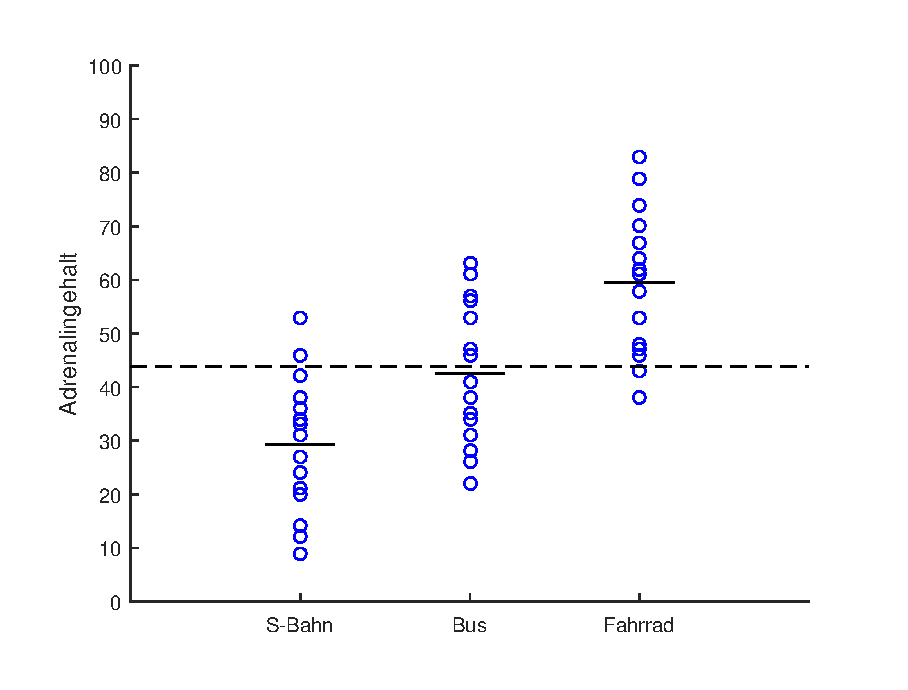
\includegraphics[width=\linewidth]{Bilder/stress}
	\end{frame}
	
	\begin{frame}{Mathematisches Modell}
		\textbf{Allgemeines Modell der einfaktoriellen Varianzanalyse} 
		\begin{center}
			\begin{tikzpicture}[thick,scale=0.8, every node/.style={scale=0.8}]
			\tikzstyle{myedgestyle} = [-triangle 60]
			
			
			\node at (-5,1.5) {$y_{k} = \mu + \alpha_k + \varepsilon_{k}$};
			\node (A1) at (-7.5,3) {Zielvariable};
			\node (A2) at (-6.4,1.8) {};
			
			\node at (-5.4,1.2)(B2) {};
			\node [align=left] (B1) at (-5.8,-0.2) {Mittelwert der\\Gesamtstichprobe};
			\node at (-4.6,1.8)(C2) {};
			\node [align=left] (C1) at (-2.8,3) {Effekt der Faktorstufe $i$\\(systematische Varianz)};
			\node at (-3.6,1.4) (D2){};
			\node [align=left] (D1) at (-0.4,1.4) {Verbleibender Fehler\\(Fehlervarianz)};
			
			
			\node at (-9.4,-2.2) {$k = 1,\dots ,K, n =1,\dots,N_k$};
			\node at (-9.6,-2)(E2) {};
			\node [align=left] (E1) at (-10,-0.8) {Anzahl der Faktorstufen des\\betrachteten Faktors};
			\node (F2) at (-7.4,-2.2) {};
			\node [align=left] (F1) at (-4,-2.4) {Stichprobenumfänge f\"ur\\die einzelnen Faktorenstufen};
	
			\draw [myedgestyle] (A1) -- (A2);
			\draw [myedgestyle] (B1) -- (B2);
			\draw [myedgestyle] (C1) -- (C2);
			\draw [myedgestyle] (D1) -- (D2);
			\draw [myedgestyle] (E1) -- (E2);
			\draw [myedgestyle] (F1) -- (F2);
			
			
			\end{tikzpicture}
		\end{center}
	\end{frame}
	
		\begin{frame}{Mathematisches Modell}
			\textbf{Allgemeines Modell der zweifaktoriellen Varianzanalyse} 
			\begin{center}
				\begin{tikzpicture}[thick,scale=0.8, every node/.style={scale=0.8}]
				\tikzstyle{myedgestyle} = [-triangle 60]
				
				
				\node at (-5,1.5) {$y_{jk} = \mu + \alpha_j  + \beta_k + (\alpha\beta)_{jk}+ \varepsilon_{jk}$};
				\node (A1) at (-9.8,2.2) {Zielvariable};
				\node (A2) at (-7.6,1.6) {};
				
				\node (B2) at (-6.5,1.2) {};
				\node [align=left] (B1) at (-7.2,-0.5) {Mittelwert der\\Gesamtstichprobe};
				\node (C2) at (-5.8,1.8) {};
				\node [align=left] (C1) at (-6,3.6) {Effekt der Faktorstufe $i$\\(systematische Varianz A)};
				\node (D2) at (-2.4,1.4) {};
				\node [align=left] (D1) at (1,1.4) {Verbleibender Fehler\\(Fehlervarianz)};
				
				\node (G2) at (-4,1.4) {};
				\node[align=left] (G1) at (-2.8,-0.6) {Interaktionseffekt zw. der Stufe $j$\\
					UVA und der Stufe $k$ UVB\\(systematische Varianz AxB)};
				
				\draw [myedgestyle] (A1) -- (A2);
				\draw [myedgestyle] (B1) -- (B2);
				\draw [myedgestyle] (C1) -- (C2);
				\draw [myedgestyle] (D1) -- (D2);
				\draw [myedgestyle] (G1) -- (G2);
				
				\end{tikzpicture}
			\end{center}
		\end{frame}
		
		\begin{frame}{Hypothesen}
			\begin{block}{einfaktoriell}
				\begin{itemize}\itemsep=2ex
					\item Nullhypothese:\\
					Alle Mittelwerte sind gleich oder alle Effekte $\alpha_k$ sind 0.\\
					Formal: $H_0: \mu_1 = \mu_2 = \dots = \mu_k$ oder $\sum\alpha_k^2=0$
					\item Alternativhypothese:\\
					Nicht alle Mittelwerte sind gleich oder mindestens ein Effekt $\alpha_i$ ist ungleich Null.\\
					Formal: $H_1: \sum(\mu_k-\mu)^2 > 0$ oder $\sum\alpha_k^2>0$
				\end{itemize}
			\end{block}
		\end{frame}
		
		\begin{frame}{Hypothesen}
			\begin{block}{zweifaktoriell}
				Für jeden Faktor wird eine Nullhypothese überprüft
				\begin{itemize}\itemsep=1ex
					\item Faktor A:\\
					Alle Zeilenmittelwerte sind gleich oder alle Effekte $\alpha_j$ sind 0.\\
					Formal: $H_0: \mu_{1\cdot} = \mu_{2\cdot} = \dots = \mu_{J\cdot}$ oder $\sum\alpha_j^2=0$
					\item Faktor B:\\
					Alle Spaltenmittelwerte sind gleich oder alle Effekte $\beta_k$ sind 0.\\
					Formal: $H_0: \mu_{\cdot1} = \mu_{\cdot2} = \dots = \mu_{\cdot K}$ oder $\sum\beta_k^2=0$
					\item Interaktion AB:\\
					Die Wirkung der einzelnen UVn auf die AV ist voneinander abhängig.\\
					Formal: $H_0: \bar{y}_{jk} = \mu_{\cdot k} + \mu_{j\cdot} - \mu + \varepsilon$
				\end{itemize}
			\end{block}
		\end{frame}
		\begin{frame}{Zweifaktorielle Varianzanalyse}
			
			\begin{table}[]
				\centering
				\resizebox{\textwidth}{!} {
				\begin{tabular}{|cc|c|c|c|c|c|}
					\hline
					\multicolumn{2}{|c|}{\multirow{2}{*}{}}        & \multicolumn{4}{c|}{UV B}                                                                                        & Zeilenmittel           \\
					\multicolumn{2}{|c|}{}                         & $B_1$                       & $B_2$                       & \dots                  & $B_K$                       & HE A                   \\ \hline
					\multirow{8}{*}{UV A} & \multirow{2}{*}{$A_1$} & \multirow{2}{*}{$\mu_{11}$} & \multirow{2}{*}{$\mu_{12}$} & \multirow{2}{*}{\dots} & \multirow{2}{*}{$\mu_{1K}$} & $\mu_{1\cdot}$         \\
					&                        &                             &                             &                        &                             & $= \mu + \alpha_1$     \\ \cline{2-7} 
					& \multirow{2}{*}{$A_2$} & \multirow{2}{*}{$\mu_{21}$} & \multirow{2}{*}{\dots}      & \multirow{2}{*}{\dots} & \multirow{2}{*}{\dots}      & $\mu_{2\cdot}$         \\
					&                        &                             &                             &                        &                             & $= \mu + \alpha_2$     \\ \cline{2-7} 
					& \multirow{2}{*}{\dots} & \multirow{2}{*}{\dots}      & \multirow{2}{*}{\dots}      & \multirow{2}{*}{\dots} & \multirow{2}{*}{\dots}      & $\mu_{j\cdot}$         \\
					&                        &                             &                             &                        &                             & $= \mu + \alpha_j$     \\ \cline{2-7} 
					& \multirow{2}{*}{$A_J$} & \multirow{2}{*}{$\mu_{J1}$} & \multirow{2}{*}{\dots}      & \multirow{2}{*}{\dots} & \multirow{2}{*}{$\mu_{JK}$} & $\mu_{J\cdot}$         \\
					&                        &                             &                             &                        &                             & $= \mu + \alpha_J$     \\ \hline
					Spalten-              & \multirow{2}{*}{HE B}  & $\mu_{\cdot1}$              & $\mu_{\cdot2}$              & $\mu_{\cdot k}$        & $\mu_{\cdot K}$             & \multirow{2}{*}{$\mu$} \\
					mittel                &                        & $= \mu + \beta_1$           & $= \mu + \beta_2$           & $= \mu + \beta_k$      & $= \mu + \beta_K$           &                        \\ \hline
				\end{tabular}
			}
			\end{table}
		
		\end{frame}
	\section{Prinzip der Varianzanalyse}
		
	\againframe{prinzipVA}
	
	\begin{frame}{Summe der Abweichungsquadrate}
		Repräsentiert die Unterschiedlichkeit der Werte der AV.
		Drei relevante Formen:
		\begin{itemize} \itemsep=2ex
			\item $SAQ_{Gesamt}$: Die Gesamtvariabilität.\\
			Formal: $SAQ_{Gesamt}= \sum(y - \bar{y})^2$
			\item $SAQ_{Effekt}$: auch $SAQ_{zwischen}$; Variabilität zwischen Bedingungen.\\
			Formal: $SAQ_{Effekt} = n_k \sum_{k=1}^{K} (\bar{y}_k - \bar{y})^2$ 
			\item $SAQ_{Fehler}$: auch $SAQ_{innerhalb}$; Variabilität innerhalb einer Bedingung.\\
			Formal: $SAQ_{Fehler} = \sum (y - \bar{y}_k)^2$ 
		\end{itemize}
		\begin{center}
			\textbf{Es gilt $\mathbf{SAQ_{Gesamt} = SAQ_{Effekt} + SAQ_{Fehler}}$}
		\end{center}
	\end{frame}
	
	\againframe{beispiel1}
		
	\begin{frame}{Freiheitsgrade (FG)}	
		
		Anzahl der frei variierbaren Werte oder auch \\
		Anzahl der in die SAQ eingehenden Werte
		\begin{itemize}
			\item $SAQ_{Gesamt}$: $N-1$
			\item $SAQ_{Effekt}$: $K-1$ \hspace{3em} K: Anzahl Faktorstufen
			\item $SAQ_{Effekt}$: $K \cdot (n-1)$
		\end{itemize}
		\textbf{Es gilt $\mathbf{FG_{Gesamt} = FG_{Effekt} + FG_{Fehler}}$}

	\end{frame}
	
	\begin{frame}{Mittlere Quadratsumme (MQ)}
		\begin{itemize}\itemsep=2ex
			\item Die mittlere Quadratsumme entspricht der Varianz
			\item $MQ_{Fehler}$: Schätzung der Populationsvarianz
			\item $MQ_{Effekt}$: Schätzung der Populationsvarianz wenn $H_0$ gilt
			\item Mittlere Quadratsummen sind \textbf{nicht} additiv
		\end{itemize}
		\begin{center}
			$MQ = \frac{SAQ}{FG}$
		\end{center}
	\end{frame}
	
	\begin{frame}{Bedeutung der MQ}
		\begin{itemize}\itemsep=2ex
			\item $MQ_{Effekt} = MQ_{Fehler}$: $H_0$ ist gültig
			\item $MQ_{Effekt} \gg MQ_{Fehler}$: $H_0$ ist ungültig, $MQ_{Effekt}$ enthält systematische Varianz
		\end{itemize}
		\begin{center}
			\textbf{Aber:} Wann ist $MQ_{Effekt}$ überzufällig größer als $MQ_{Fehler}$?
			\pause\\ \hfill\\ $\Rightarrow$ Prüfen mit F-Verteilung \vspace{2ex} \\
			$F = \frac{MQ_{Effekt}}{MQ_{Fehler}}, FG=K-1,K(n-1)$
		\end{center}
		
	\end{frame}
	
	\begin{frame}{F-Verteilung}
		Wenn $F_{empirisch} > F_{kritisch} \Rightarrow $ Ablehnung von $H_0$
		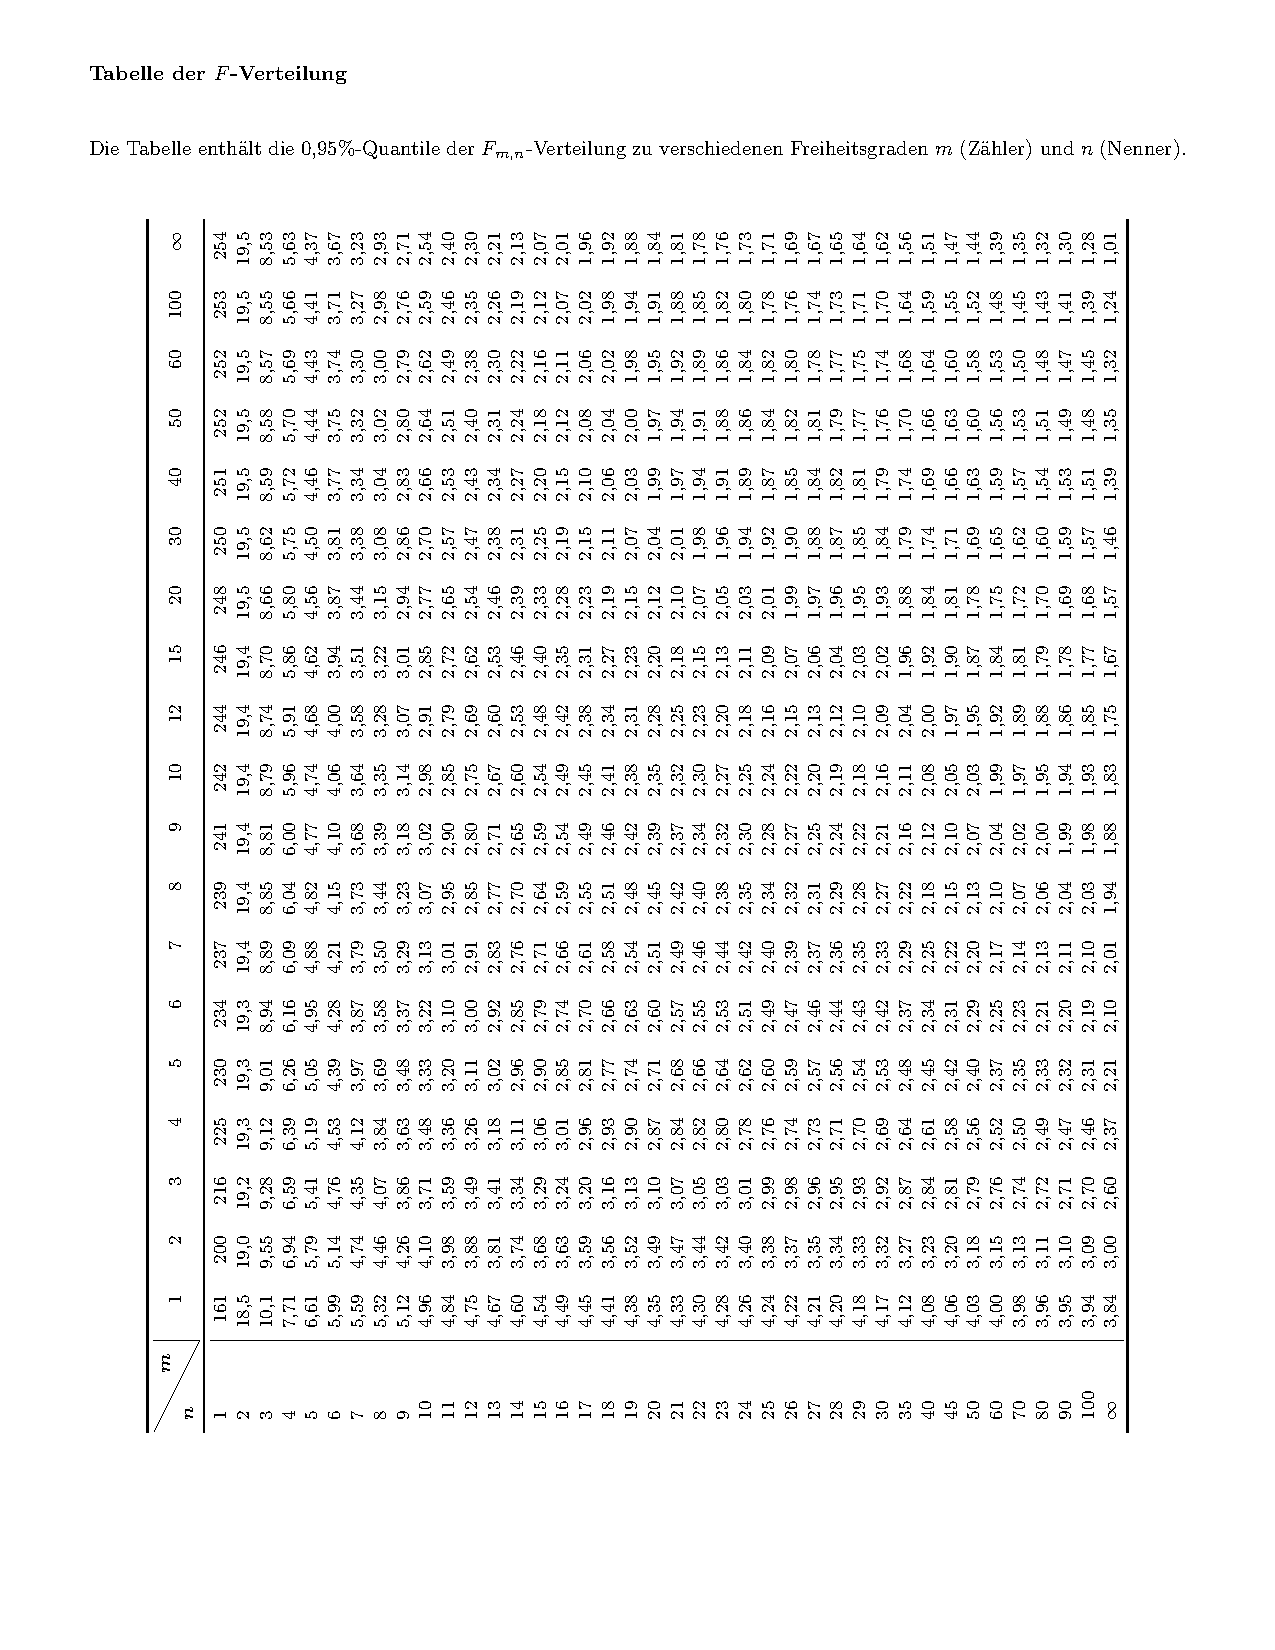
\includegraphics[trim=60 100 240 190,clip,angle=270,origin=c, width=\textwidth]{Bilder/F-verteilung}
		\let\thefootnote\relax\footnote{{\fontsize{5}{5} \selectfont \vspace{-5ex}
				Quelle: https://www.statistik.tu-dortmund.de/fileadmin/user\_upload/Lehrstuehle/Oekonometrie/Lehre/WiSo-Stat-1415/tabelleF.pdf}}
	\end{frame}
	
	
	\section{Robert}
	
	
	%---------------------------------- Ab hier Beispiele für Folien
	
	\section{Historische Einordnung}
	
	\begin{frame}{Beginn des Schlangenöls}
		\begin{columns}[T,onlytextwidth]
			\column{0.7\textwidth}
			\begin{itemize}
				\item aus Mythologie des Wilden Westens
				\item von Wunderheilern eingesetzt
				\item Heilmittel für Gebrechen aller Art
			\end{itemize}
			
			%------------------------ Bilder
			\column{0.3\textwidth}
				
\includegraphics[width=1\textwidth]{Bilder/snakeoil.jpeg}
			%------------------------ Bilder

		\end{columns}
	\end{frame}
	
	\begin{frame}{Schlangenöl allgemein}
		\begin{itemize}
			\item versprochenes Wundermittel
			\item unübersichtliche Bereiche, oft in Technik
			\item \alert{wenig Wirkung}
			\item Heutige Anwendungen oft in Kryptografie und \alert{Antiviren-Software}
		\end{itemize}
	\end{frame}
	
	\section{Malware und ihre Hauptverteilwege}
	
	\begin{frame}{Malware}
		\begin{alertblock}{Malware}
			Software, welche schädliche Funktionen ausführen
		\end{alertblock}
		
		\begin{itemize}
			\item Viren
			\item Würmer
			\item Trojanische Pferde
			\item Ransomware 
			\item ...
			\item \alert{nicht:} fehlerhafte Software
		\end{itemize}
	\end{frame}
	
	\begin{frame}{Verschiedene Malware}
		\begin{alertblock}{Virus}
			Schadprogramm, welches sich verbreitet, in dem es sich in andere Software einschleust. Durch das Kopieren dieser wird der Virus passiv verbreitet (und dabei oft nur lokal)
		\end{alertblock}
		\begin{alertblock}{Wurm}
			Schadprogramm, welches sich aktiv ausbreitet, in dem es Sicherheitsprobleme ausnutzt. Für Nutzer kaum unterschiedlich zu Viren
		\end{alertblock}
		\begin{alertblock}{Trojanisches Pferd}
			Schadprogramm, welches sich als nützliche Anwendung tarnt und ohne Wisse des Anwenders (auch) schädliche Funktionen ausführt
		\end{alertblock}
	\end{frame}
	
	%------------------------ Bilder
	\begin{frame}{Anzahl Malware}
		\begin{figure}
			\centering
			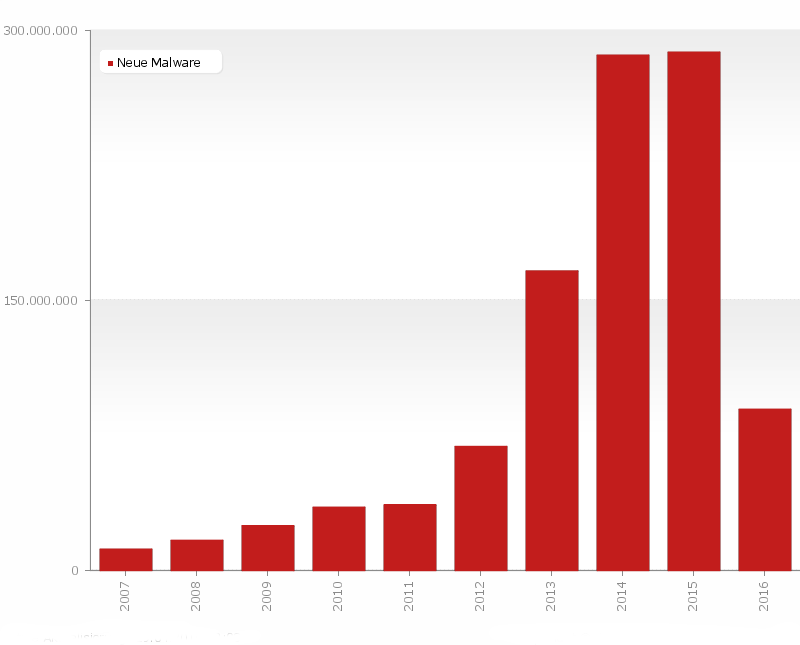
\includegraphics[width=0.7\textwidth]{Bilder/new_malware_transparent.png}
			\caption{Registrierung neuer Schadprogramme in den letzten 10 Jahren. Quelle: avtest}
		\end{figure}		
	\end{frame}
	%------------------------ Bilder
	
	\begin{frame}{Verteilwege von Malware}
		\begin{itemize}
			\item E-Mail-Dateianhänge
			\item Drive-by-Downloads
			\item Datenträger
			\item Netzwerke
		\end{itemize}
	\end{frame}
	
	\begin{frame}{Statistiken}
		\begin{alertblock}{Problem}
			Viele Statistiken zu Malware und ihren Verteilwegen werden von Antiviren-Software-Firmen angeboten
		\end{alertblock}
		\begin{itemize}
			\item wenige \alert{unabhängige} Quellen
			\item Quantität schwer einzuschätzen
			\item nur bekannte Probleme aufgelistet
		\end{itemize}
	\end{frame}
	
	
	\section{Antiviren-Programme}
	
	\begin{frame}{Vermeintliche Lösung}
		\begin{alertblock}{Wie schützen wir uns vor Viren?}
			Wir installieren ein Antiviren-Programm!
		\end{alertblock}
	\end{frame}
	
	\begin{frame}{Verbreitung von AV-Programmen}
		\begin{alertblock}{Zahlen zu AV-Installationen}
			\begin{itemize}
				\item{AVG Antivirus Free (32 \& 64 bit) 22.3M}
				\item{avast Free Antivirus 19.4M}
				\item{Ad-Aware Free Antivirus 9.2M}
			\end{itemize}
			jeweils in Millionen Downloads bei Chip (Windows)
		\end{alertblock}
	\end{frame}

	\subsection{Aufgaben und Vorgehen von AV-Programmen} %----------- Beachte: keine 
	
	\begin{frame}{Virtualisierung I}
		\begin{alertblock}{Virtualisierung}
			Idee: Wir tun nur so, als würden wir verdächtigen Code laufen lassen, überwachen tatsächlich seine Verhaltensweise
		\end{alertblock}
	\end{frame}
	
	
	\begin{frame}{Firewalls I}
		\begin{alertblock}{Firewall}
			Idee: Ein- und ausgehende Kommunikation überwachen, um Kommunikation von Malware zu verhindern/ Malware zu finden\\
		\end{alertblock}
		\begin{alertblock}{Problem}
			Sobald die Kommunikation verschlüsselt abläuft, wird die Überwachung beliebig kompliziert
		\end{alertblock}
	\end{frame}
	
	
	
	\begin{frame}{AV-Browser I}
		\begin{alertblock}{Antiviren-Browser}
			Idee: Wir halten den Nutzer davon ab, schädliche Dateien herunterzuladen, indem wir einen Browser bereitstellen, der gefährliche Websites u.Ä. blockiert
		\end{alertblock}
	\end{frame}
	
	
	\section{Wirksame Maßnahmen gegen Viren}
	
	
	\begin{frame}{Zitat}
		\glqq We cant write secure software. Why are people suprised that we also can not write secure security software?\grqq
	\end{frame}
	
	\begin{frame}[standout]
		Fragen?
	\end{frame}
	
	\appendix
	
	
	\begin{frame}[allowframebreaks]{Quellen}
		\footnotesize
		%\bibliography{demo}
		%\bibliographystyle{abbrv}
		\begin{itemize}
			\item blog.fefe.de
			\item sherpablog.marketingsherpa.com/wp-content/uploads/2016/02/Snake-Oil-Cures-All.jpeg
			\item itwissen.info/definition/lexikon/ (diverse Definitionen)
			\item de.wikipedia.org/wiki/Schadprogramm
			\item av-test.org/de/statistiken/malware/
			\item netmarketshare.com/operating-system-market-share.aspx?qprid=10\&qpcustomd=0
			\item bsi.bund.de/DE/Publikationen/Lageberichte/bsi-lageberichte.html
			%ab hier robads
			\item Chip.de (diverse AV-Downloadseiten)
			\item bugs.chromium.org/p/project-zero/issues/detail?id=769
			\item de.urbandictionary.com/define.php?term=Startkeylogger 
			\item bugs.chromium.org/p/project-zero/issues/detail?id=564\&redir=1
			\item news.softpedia.com/news/avast-safezone-browser-lets-attackers-access-your-filesystem-499990.shtml
			\item imgur.com/Smwnzx3
			\item www.heise.de/security/meldung/Authentifikation-von-McAfees-Enterprise-Security-Manager-loechrig-3036068.html
			\item www.heise.de/security/meldung/Symantec-Endpoint-Protection-Gefaehrlicher-Sicherheitsluecken-Cocktail-2768461.html
			\item thehackernews.com/2015/07/bitdefender-hacked.html?m=1
			\item www.heise.de/mac-and-i/meldung/Apple-Anti-Viren-Apps-fuer-iOS-irrefuehrend-2581916.html
			\item www.heise.de/security/meldung/Antiviren-Software-und-Apples-Schutzmechanismen-fuer-Mac-OS-X-nutzlos-2620049.html
		\end{itemize}

		
	\end{frame}
	
	
	
\end{document}